\documentclass[11pt]{article}
\usepackage[left=3cm, right=3cm, top=2cm, bottom=2cm]{geometry}
\usepackage{amsmath}
\usepackage{amsfonts}
\usepackage{multirow}
\usepackage{graphicx}
\usepackage{enumitem}
\usepackage{subfig}

\title{6.047 Problem Set 2 Writeup}
\author{Matthew Feng}
\date{\today}

\begin{document}

\maketitle
\section{Naive Bayes}
\subsection*{(a) Naive Bayes Assumption}
No, the naive Baye's assumption that the features
are independent conditioned on the class does not hold
in this case. This is because the complexity of the
sequence is likely dependent on the length of the
sequence, as well as the GC content. If the GC content
of a sequence is high, then the sequence is more likely
to be a CpG island, which would mean that the complexity
is lower because of the repeated base ordering.

\subsection*{(b) Computing MLEs}

\paragraph{Maximum Likelihood Estimates}

\begin{center}
\begin{tabular} { l | l  l  l }
& $X_1$ & $X_2$ & $X_3$ \\
\hline
\multirow{3}{6em}{$P(\ \cdot\ |\ repeat)$}
& $0$, short & $0$, low content    & $2/3$, low complexity \\
& $1$, long  & $0$, medium content & $1/3$, high complexity\\
&            & $1$, high content   & \\
\hline
\multirow{3}{6em}{$P(\ \cdot\ |\ gene)$}
& $0$, short & $2/3$, low content    & $1/3$, low complexity \\
& $1$, long  & $1/3$, medium content & $2/3$, high complexity\\
&            & $0$,   high content   & \\
\hline
\multirow{3}{6em}{$P(\ \cdot\ |\ motif)$}
& $1$, short & $0$,   low content    & $1/4$, low complexity \\
& $0$, long  & $1/2$, medium content & $3/4$, high complexity\\
&            & $1/2$, high content   & \\
\end{tabular}
\end{center}

\paragraph{Prior probability distribution}
\[
P(Y) = 
\begin{cases}
    $3/10$, & Y = repeat \\
    $3/10$, & Y = gene \\
    $4/10$, & Y = motif \\
\end{cases}
\]

\subsection*{(c) Predicted MAP Class}

The maximum a posteriori estimate of class of
$(X_1, X_2, X_3) = (long, medium, low)$ is $Y = gene$;
we don't need to compute the denominator of 
Baye's theorem for two reasons: the other classes have
probability of $0$ in the numerator, and that the
MAP estimate of class is proportional only to the
numerator; the denominator is just a normalization
factor that is the same for all classes. Therefore, 
if we are only doing classification, we can just
compare proportions rather than exact values.

\begin{align*}
P(Y | X_1, X_2, X_3)
&= \dfrac{P(X_1, X_2, X_3 | Y)P(Y)}{P(X_1, X_2, X_3)}
& \text{(Baye's theorem)}\\
&= \dfrac{P(X_1 | Y)P(X_2 | Y)P(X_3 | Y)P(Y)}{P(X_1, X_2, X_3)}
& \text{(Naive Baye's assumption)}\\
\end{align*}

\section{Classification of Conserved Regions}
\subsection*{(a) Conditional probabilities}
\paragraph{Alignment 1}
$\log \mathbb{P}(S | N) = -17.098$,
$\log \mathbb{P}(S | C) = -24.177$

\paragraph{Alignment 2}
$\log \mathbb{P}(S | N) = -17.504$, 
$\log \mathbb{P}(S | C) = -13.256$

\subsection*{(b) Classification error I}
The classification error, or amount of time that $P(S | C) > P(S | N)$
even though $S$ is sampled from $N$, is $0.128$ ($12.8\%$).

\subsection*{(c) Classification error II}
The classification error, or amount of time that $P(S | N) > P(S | C)$
even though $S$ is sampled from $C$, is $0.1412$ ($14.1\%$).

\subsection*{(d) Reduce classification error}
\subsubsection*{(i) Good discriminators}
Score values $1$ and $6$ are good discriminators between the two models,
because of the difference between the relative frequencies is high.

\subsubsection*{(ii) Bad discriminators}
Score values $2$ and $3$ are poor discriminators between the two models,
because of the difference between the relative frequencies is low.\\

The rate of classification errors would not decrease if
we dismissed alignment scores of $0$, because
$0$ is a good discriminator; alignments of $0$
are twice as likely to occur in model $N$ than in
model $C$.

\subsection*{(e) Long sequences}
We can reduce the classification errors for longer sequences by
splitting them into shorter sequences, so that the whole
sequence is not necessarily classified as a single class.
Additionally, if we split the long sequence into
shorter segments but compute the classification
probabilities multiple times with the breaks at different locations,
then we can further improve accuracy by checking which segments are
classified as a certain class consistently throughout the
different segmentations.

\section{K-means Clustering}
\subsection*{(a) $k$-means implementation}
See {\tt kmeans.py}.
\subsection*{(b) {\tt tissue1} results}
See Figure 1.
\begin{figure}
\begin{tabular}{c c}
    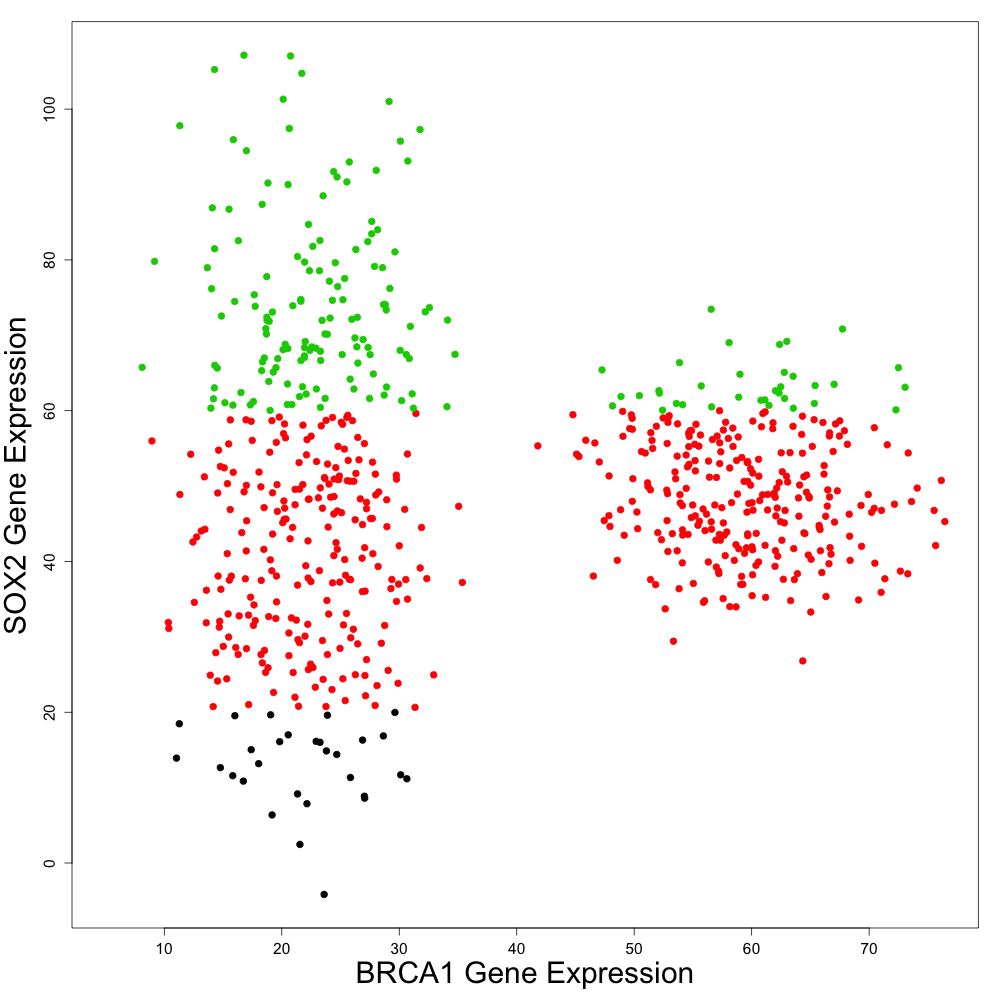
\includegraphics[width=65mm]{../tissue1_plots/cluster_step1.png} & 
    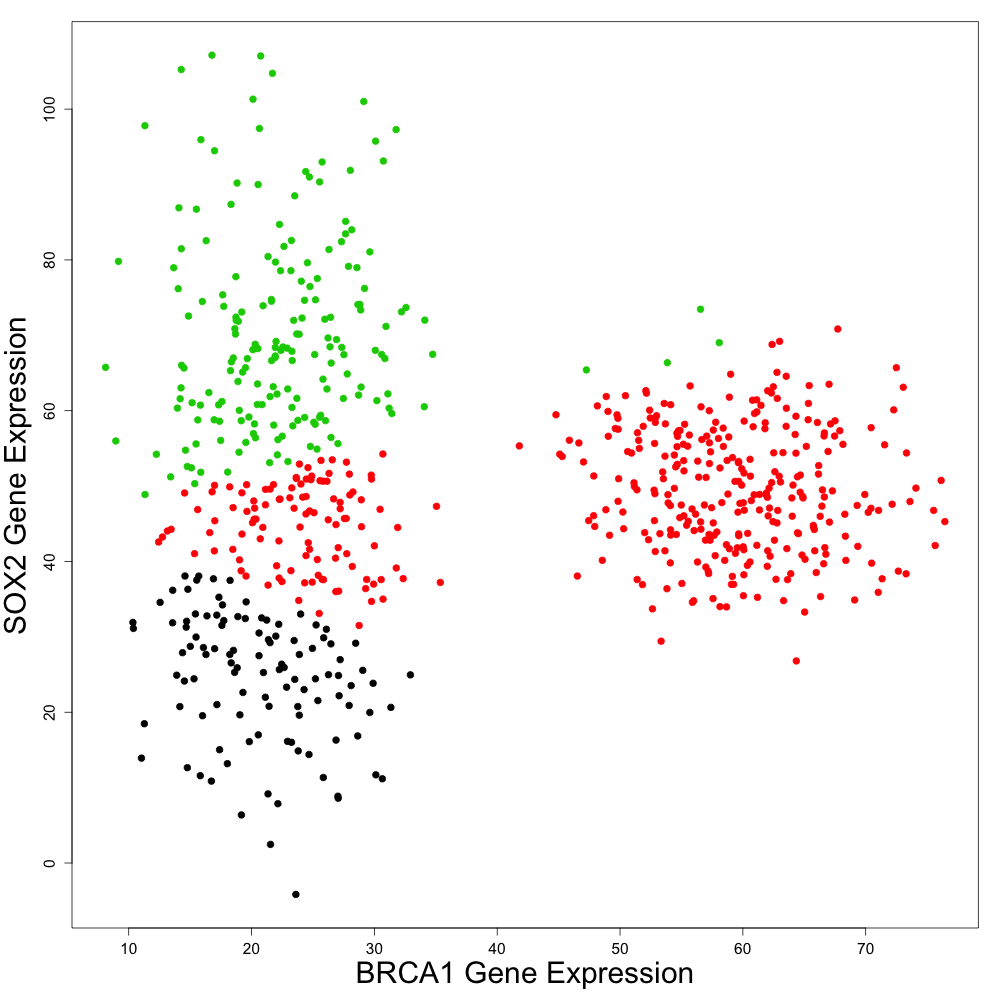
\includegraphics[width=65mm]{../tissue1_plots/cluster_step2.png} \\
    (a) Step 1 & (b) Step 2 \\
    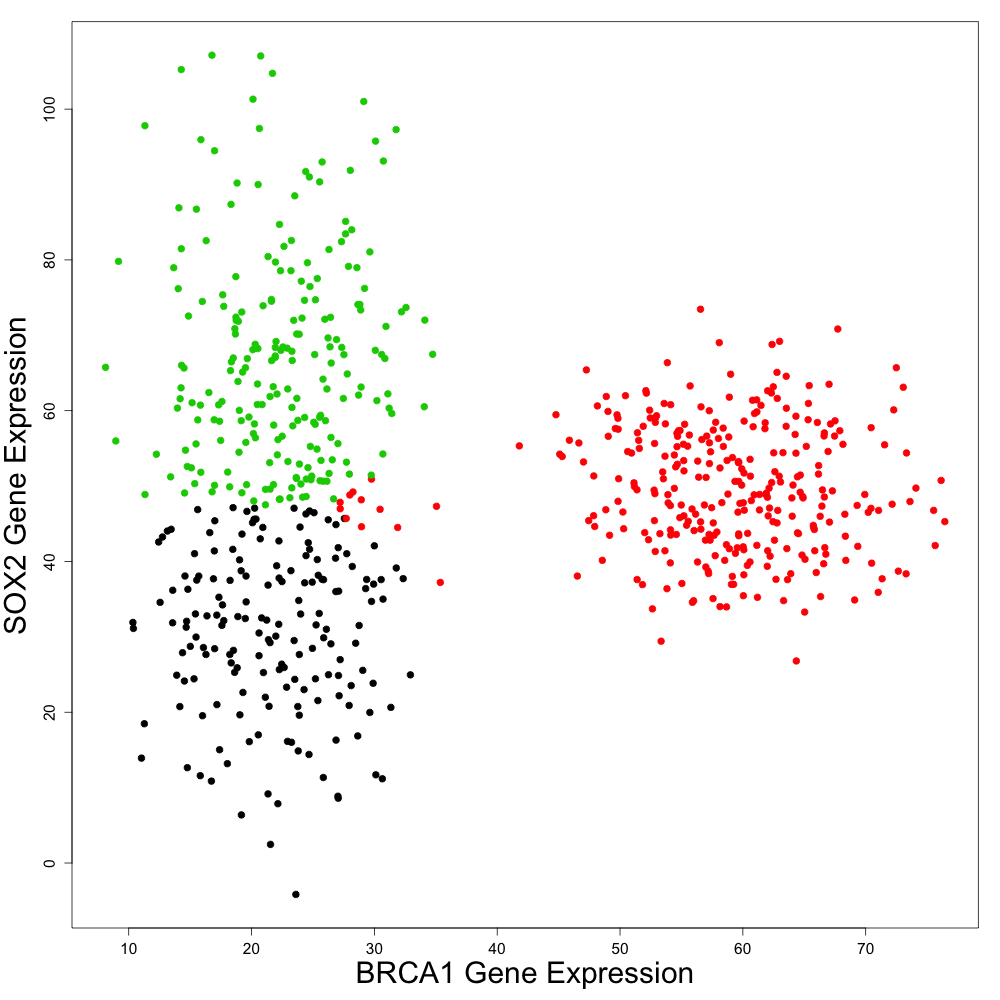
\includegraphics[width=65mm]{../tissue1_plots/cluster_step3.png} & 
    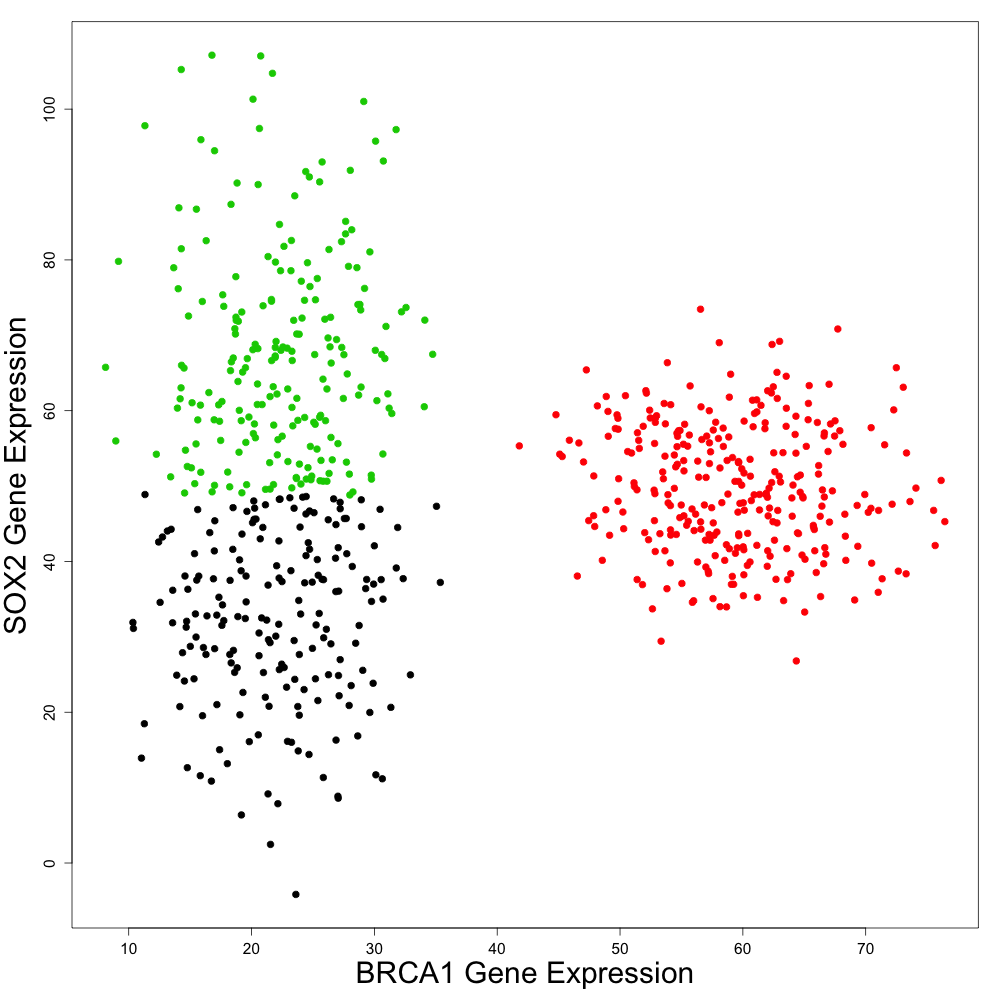
\includegraphics[width=65mm]{../tissue1_plots/cluster_step4.png} \\
    (c) Step 3 & (d) Step 4 \\
\end{tabular}
\caption{Four steps of convergence for the $k$-means algorithm
on {\tt tissue1\_data.txt}.}
\end{figure}

\subsection*{(c) Improving $k$-means}
See Figures 2 and 3. One of the flaws of $k$-means clustering is
that it doesn't always find the most obvious clusters if the
initial guesses for the centroid are not good. If we look at
Figure 2, we can see that the clusters that were found were biased
by the initial guesses for the centroids, which led the algorithm
to find oddly-shaped clusters instead of the ``obvious'' ones that
we see with our own eyes. In order to remedy
this problem, it is beneficial to run $k$-means with random initialization,
meaning that the initial guesses for the centroids are randomly
placed in the feature space. In particular, $k$-means can be improved
by running many times with random initialization, and then using
the clustering that has the lowest average distance to the centroids.

\begin{figure}
\begin{tabular}{c c}
    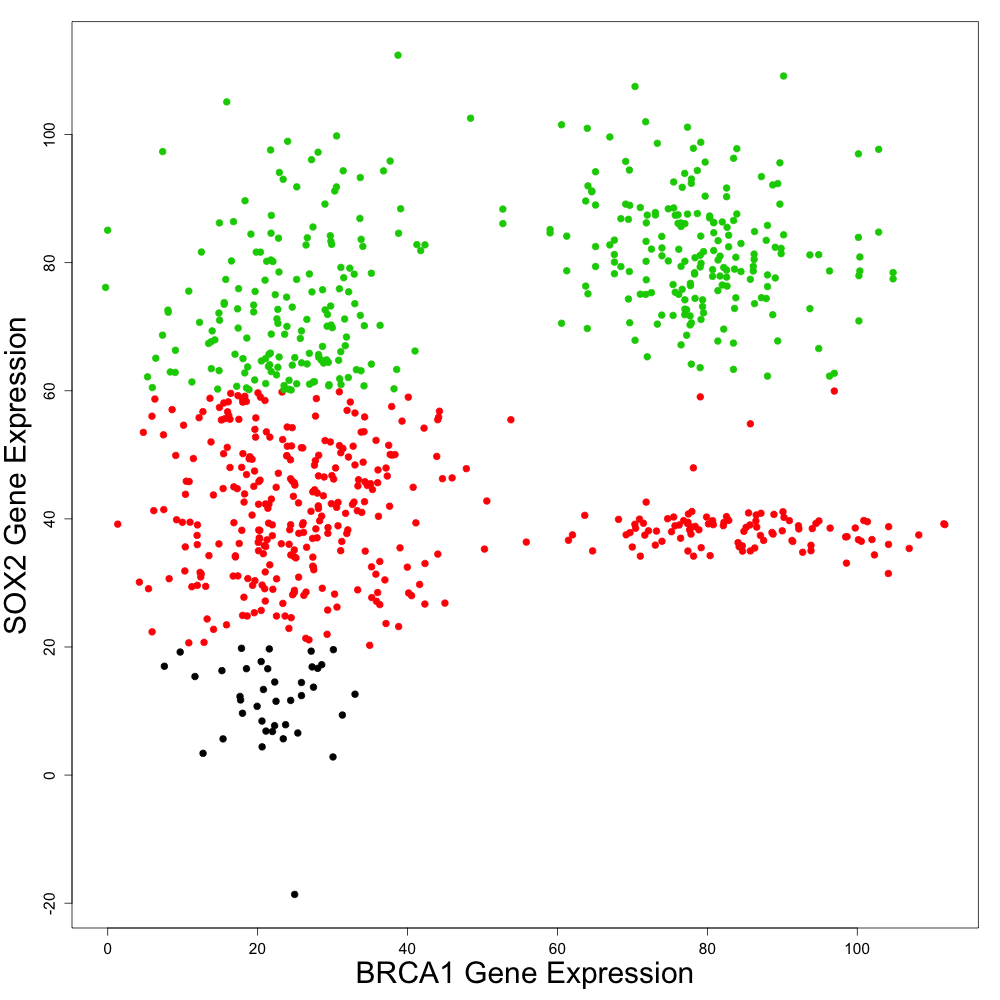
\includegraphics[width=65mm]{../tissue2_plots/cluster_step1.png} & 
    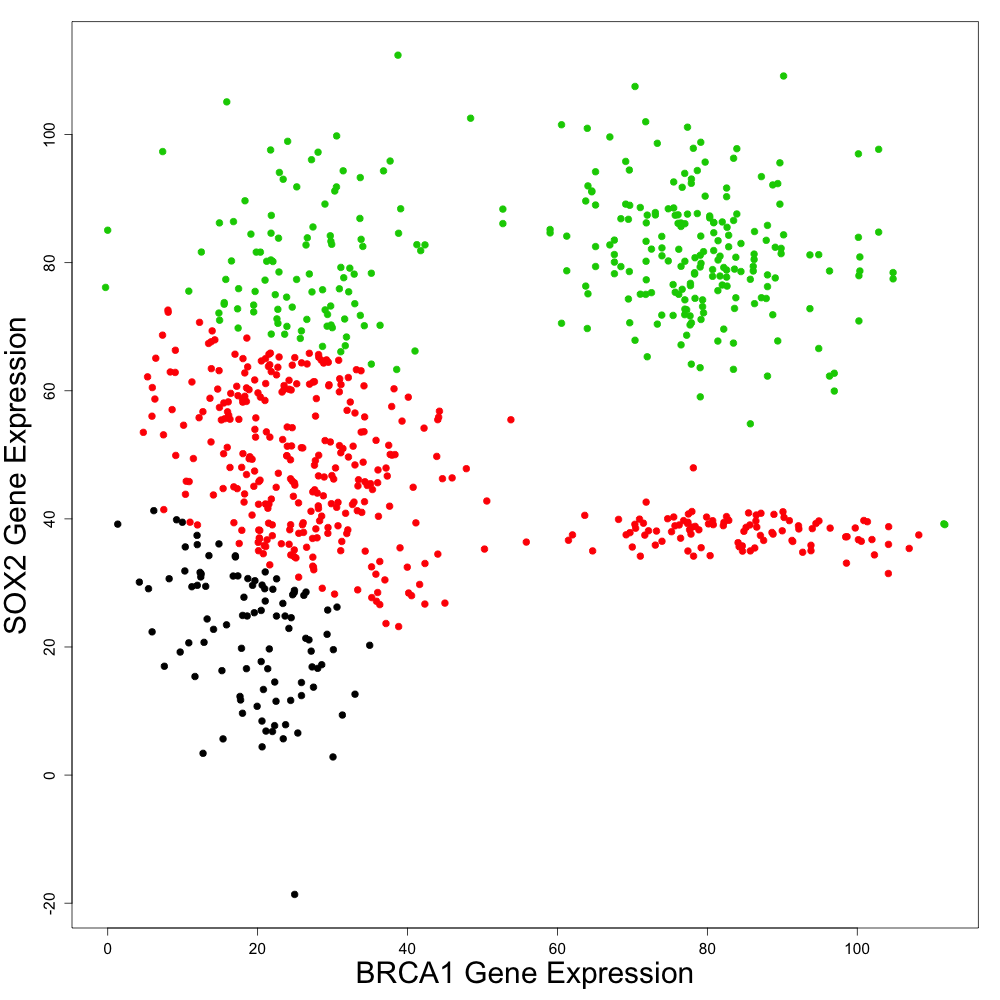
\includegraphics[width=65mm]{../tissue2_plots/cluster_step2.png} \\
    (a) Step 1 & (b) Step 2 \\
    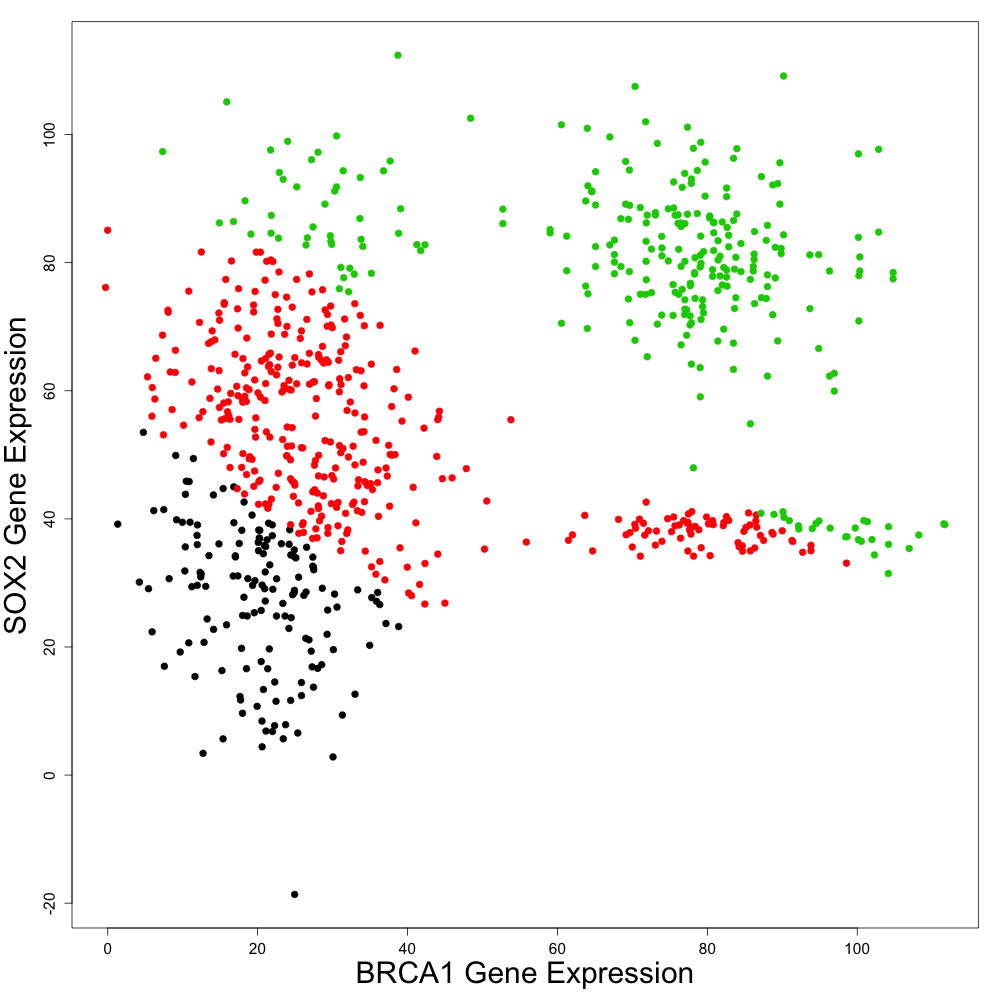
\includegraphics[width=65mm]{../tissue2_plots/cluster_step3.png} & 
    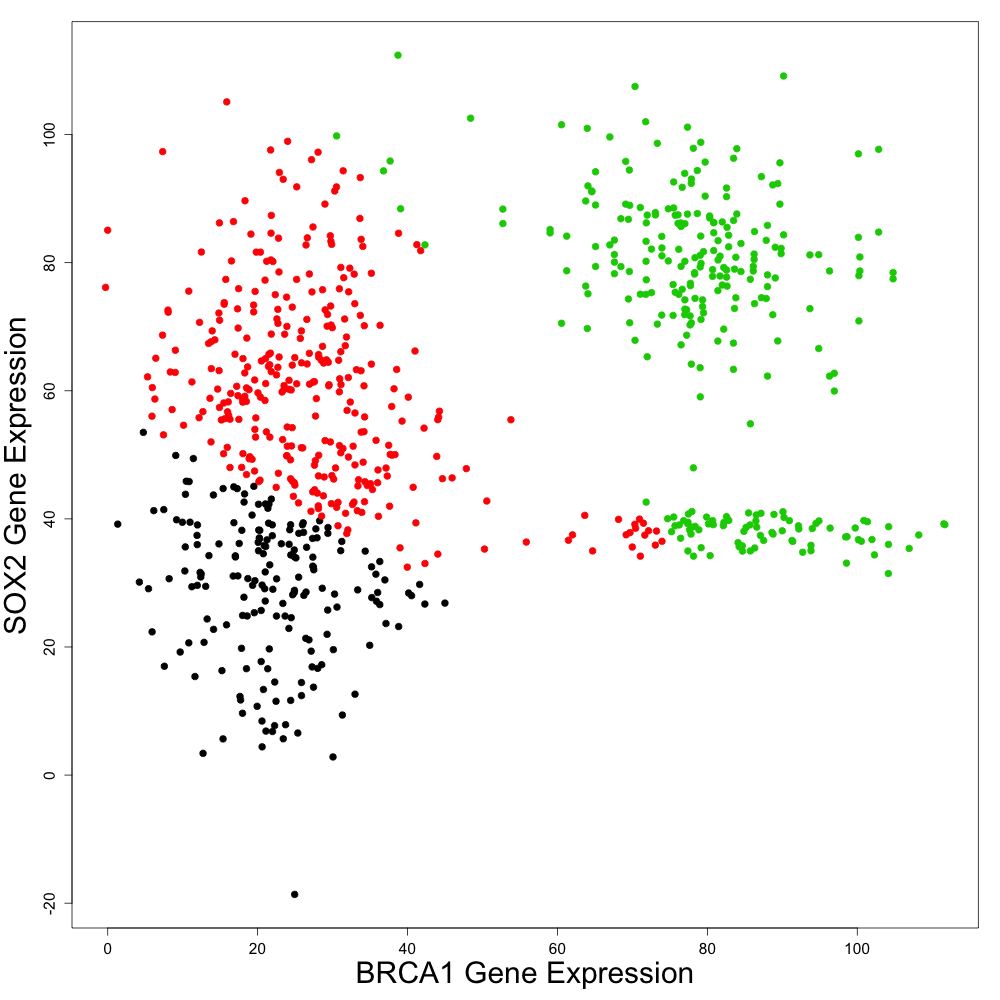
\includegraphics[width=65mm]{../tissue2_plots/cluster_step4.png} \\
    (c) Step 3 & (d) Step 4 \\
    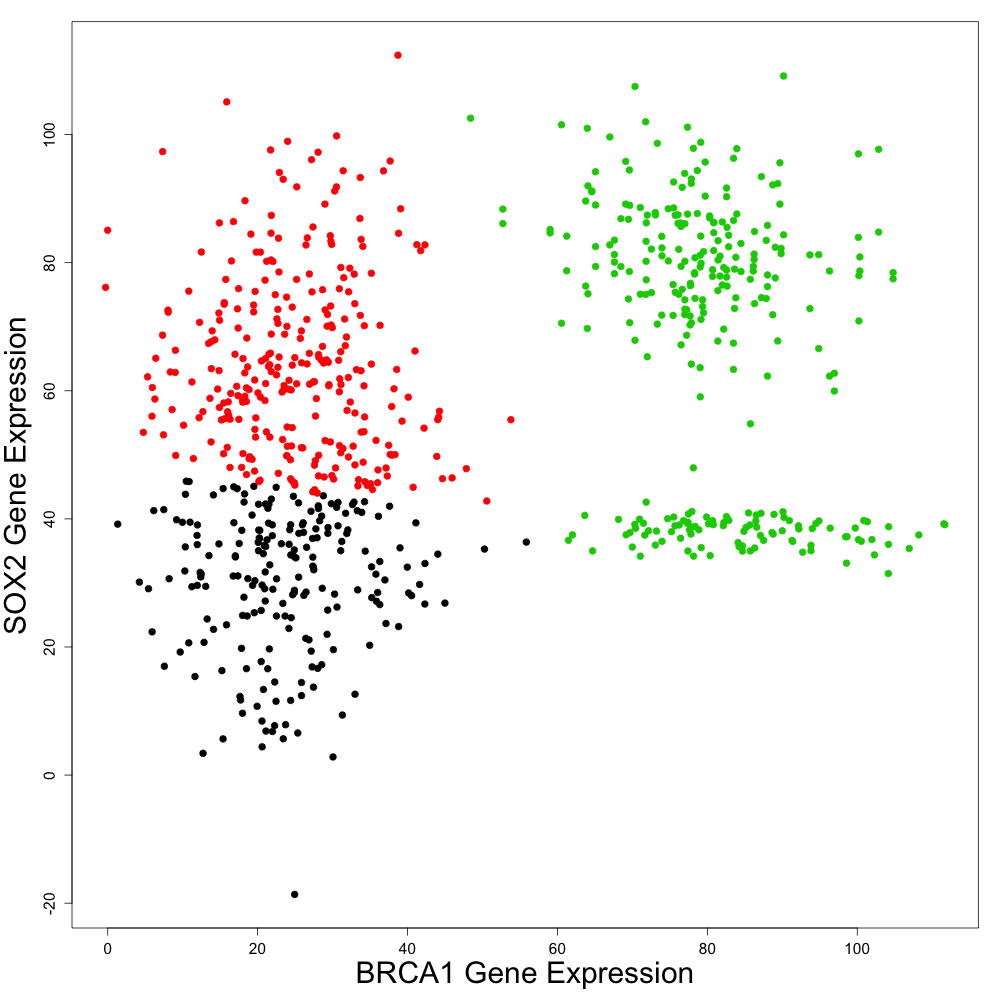
\includegraphics[width=65mm]{../tissue2_plots/cluster_step5.png} & 
    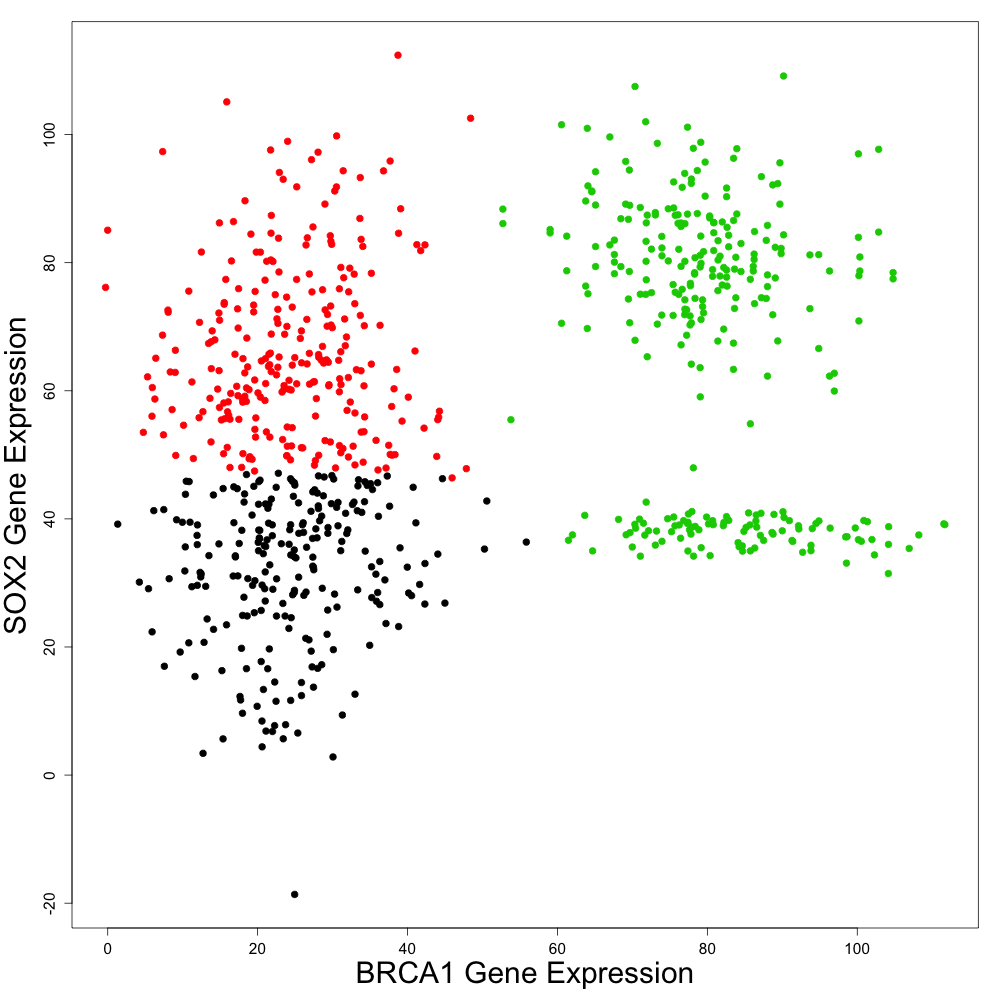
\includegraphics[width=65mm]{../tissue2_plots/cluster_step6.png} \\
    (c) Step 5 & (d) Step 6 \\
\end{tabular}
\caption{Six steps of convergence for the $k$-means algorithm
 on {\tt tissue2\_data.txt}.}
\end{figure}

\begin{figure}
\begin{tabular}{c c}
    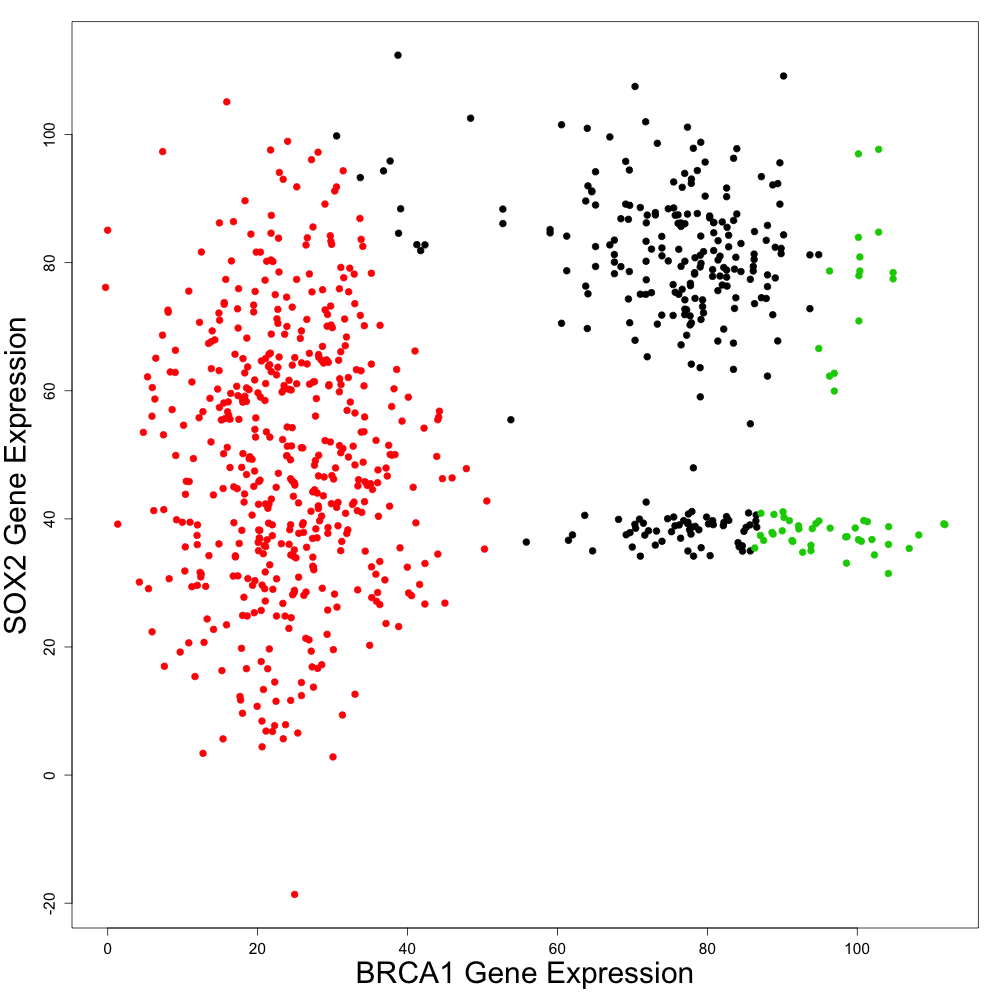
\includegraphics[width=65mm]{../tissue2random_plots/cluster_step1.png} & 
    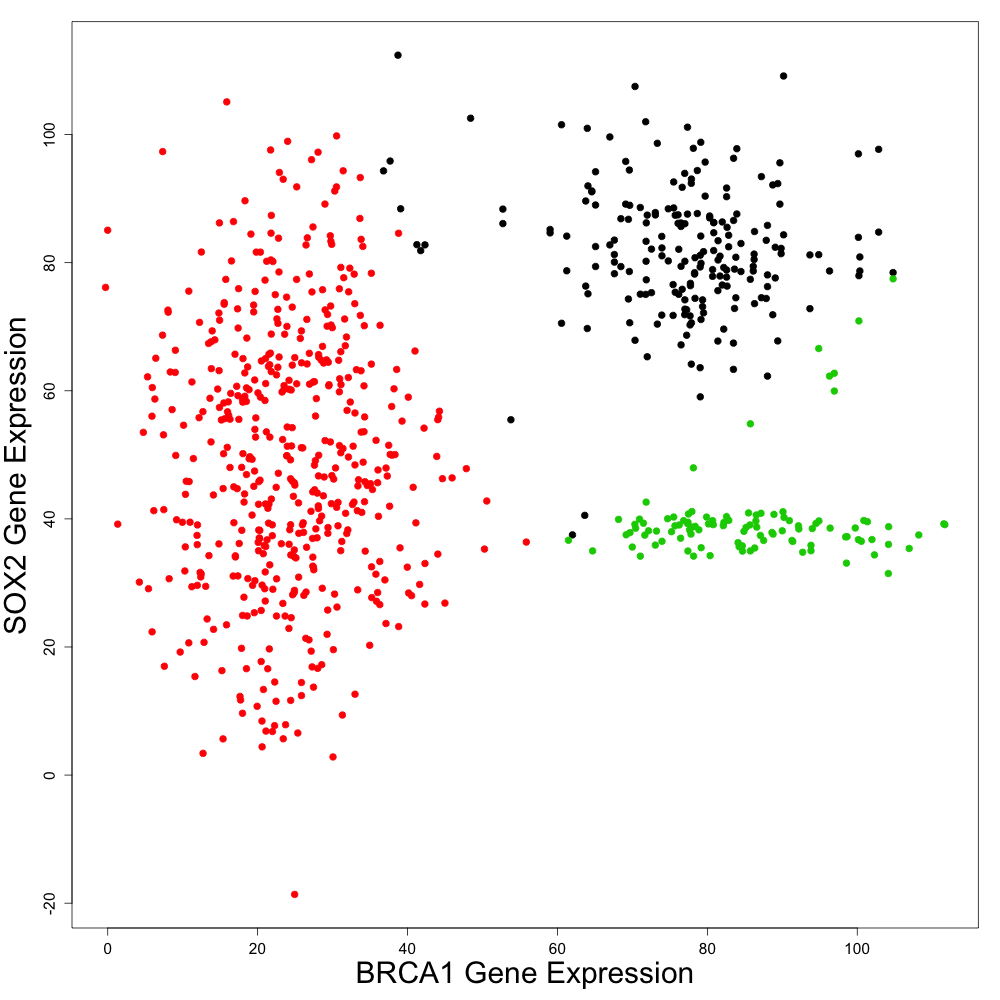
\includegraphics[width=65mm]{../tissue2random_plots/cluster_step2.png} \\
    (a) Step 1 & (b) Step 2 \\
    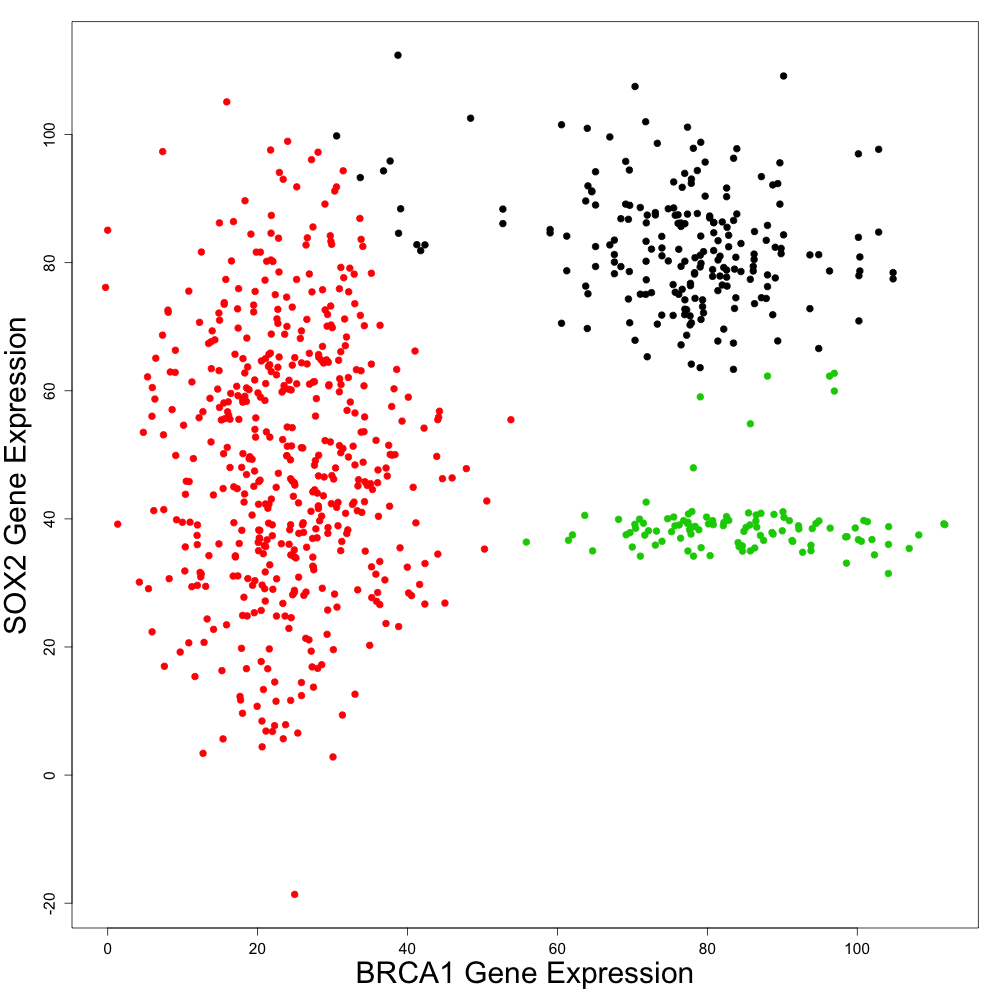
\includegraphics[width=65mm]{../tissue2random_plots/cluster_step3.png} & \\
    (c) Step 3 & \\
\end{tabular}
\caption{Three steps of convergence for the $k$-means algorithm 
with random initialization on {\tt tissue2\_data.txt}.}
\end{figure}

\subsection*{(d) Fuzzy $k$-means}
We can implement fuzzy $k$-means by assigning to each point in our
dataset not a class, but a probability that it belongs to a certain
class. We can do so by computing the probability that a certain
point belongs to a cluster via a normal distribution (farther away
is less probable, with a Gaussian probability dropoff). When we
update the location of the centroids, we compute the weighted average
of all the data points, with the weight of contribution for each
data point weighted by the probability it belongs to the cluster.
See {\tt fuzzykmeans.py} for the implementation.

We could graphically represent the fuzzy clusters by mixing RGB colors;
class 1 could be encoded as red, class 2 as green, and class 3 as blue.
Depending on the probability that the point belongs do class $i$, we could
use function (the CSS function) {\tt rgb(r, g, b)} to find a representative
color for the probabilities.

\section{Final project preparation}
\subsection*{(b) Evaluate proposals}
What do you find most exciting about the proposal?
What would you do differently for that proposal?
What aspects of the area did the proposal leave unaddressed, and how would you address them?

\subsubsection*{Representation learning for microbial genes and genomes}
Relevant file: {\tt anon23.pdf}\\
Natural language processing is very exciting in that although the field
was originally designed to handle spoken languages from across the globe,
it has evolved to apply to any language that we used, from scientific disciplines
to historical languages to mathematical logic. Surprisingly, NLP algorithms
work very well, and the theory extends beyond the languages we commonly
see. As such, this project proposal is very exciting because it attempts to
apply word embeddings, in particular {\it lda2vec} word embeddings, in
order to learn relationships amongs microbial gene sequences.

One shortcoming of the proposal is that it doesn't specify any metric for
measuring the success of their technique; I would make a modification that
would include some metric that allows the results to be quantified, beyond
using examples as evidence that the embeddings have some more meaning
behind them.

The proposal doesn't address how these word embeddings could be used;
designing an extension that tries to use word embeddings as a feature set
for prediction would also allow for more interesting applications and
insight into the microbial gene language.

\subsubsection*{Inferring non-canonical metabolic pathways to improve cancer tissue classification}
Relevant file: {\tt anon12.pdf}\\
The proposal is exciting because it extends a novel algorithm and applies it
to other deviations that cancer introduces from the ``canonical'' pathways
known for healthy cells. In addition to examining uncommon metabolic pathways,
the project proposed will also examine aberrant gene methylation, and try
to extract features from these other areas in order to better classify 
cancer tissue.

The proposal doesn't address how their proposed unsupervised learning
techniques would identify these unknown features; I would be more
specific or use the same unsupervised learning techniques as the MCF authors
did, in order to be able to best understand the results.

\subsection*{(c) Evaluate scientific papers}

\subsubsection*{Development and Validation of a Deep Learning Algorithm for
Detection of Diabetic Retinopathy in Retinal Fundus Photographs}
This paper is exciting because it is one of the first demonstrations of the
validity and applicability of convolutional neural networks to radiology.
The authors do not propose such a system to replace radiologists, but rather
as a substantial aid to reduce the number of false-negatives that may have
gone unnoticed otherwise.

The authors leave for further research how to translate the predictive
abilities of the convolutional neural network into human understandable
insights to improve radiologist performance in detecting diabetic retinopathy.
The main reason this area is untouched is the extreme complexity that neural
networks bring, and the opaqueness of their logic currently. Augmenting such
a system with some technique that could give rationale for decisions would
not only further human understanding of radiology, but also add confidence
to those who use the system.

I would attempt to address this adding a requirement to the neural network
that forces it to label regions that it believes are important, and then
train a convolutional neural network on the labeled regions to output
whether or not an image indicates diabetic retinopathy. The inspiration
for such a network stems from Barzilay's paper, ``Rationalizing Neural
Predictions'', which uses a similar approach.

\subsubsection*{Data-Driven Metabolic Pathway Compositions Enhance Cancer Survival Prediction}
What I find most exciting about this paper is the implementation of a well
known fact that cancer cells have unique metabolic pathways into a system
that attempts to find such paths on training data, and then apply those paths
to testing data to classify cell type. It is a novel approach of mixing
unsupervised learning algorithms with traditional graph search algorithms
in order to identify new features for supervised learning.

The authors have left open the problem of improving the MCF algorithm via
better heuristics for computing the longest path, which is well known to be
a NP-complete problem. Furthermore, the researchers have not yet tried to use
their MCF algorithm to explore the different metabolic pathways that
cancer cells construct, separate from the application of these pathways as
predictive characteristics of cancer.

The researchers have also not published the code that they wrote that
constructed these MCF pathways; to address this issue, I would try to
implement the algorithm based on their discussion and see whether or
not the results are reproducible.

\subsection*{(d) Project idea}
A project I had would be to extend upon DeepMind's paper on
diabetic retinopathy to incorporate rationalization and reasoning
as to what the neural network ``saw'' when deciding a classification for
the patient.

I would need to gather the training and testing data that was used
for the DeepMind paper, as well as pixel masks that highlight what
expert radiologists believed to be key factors in determining the
class for a sample image. I would also need very strong compute
capabilities, as training on images is very computationally expensive.
However, I believe that the approach can yield insights into where
the neural network pays attention in an image, and improve upon
our understanding of radiology.

One of the challenges I anticipate is making sure the neural network
converges, along with making sure that the pixel selection process is
differentiable, in order for the network to be able to train. Furthermore, 
determining the appropriate hyperparameters for the model to tune it will
take time as well.

\subsection*{(e) Potential project partners}
\begin{itemize}[noitemsep]
\item Chris Giuliano
\item Peter Wang
\item Soumya Kannan
\end{itemize}

\end{document}